\documentclass{standalone}
\usepackage{xcolor}
\usepackage{verbatim}
\usepackage[T1]{fontenc}
\usepackage{graphics}
\usepackage{hyperref}
\newcommand{\code}[1]{\texttt{#1}}
\newcommand{\R}{R}
\newcommand{\pkg}[1]{#1}
\newcommand{\CRANpkg}[1]{\pkg{#1}}%
\newcommand{\BIOpkg}[1]{\pkg{#1}}
\usepackage{amsmath,amssymb,array}
\usepackage{booktabs}
\usepackage{mathtools}
\usepackage{algorithm}
\usepackage{threeparttable}
\usepackage[noend]{algpseudocode}
\makeatletter
\def\BState{\State\hskip-\ALG@thistlm}
\makeatother
\usepackage{tikz}
\begin{document}
\nopagecolor
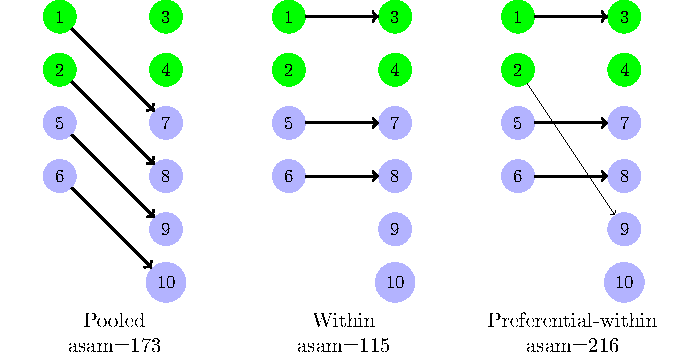
\includegraphics{tikz/matcha.pdf}
\begin{verbatim}
\minipage{0.32\textwidth}
\centering
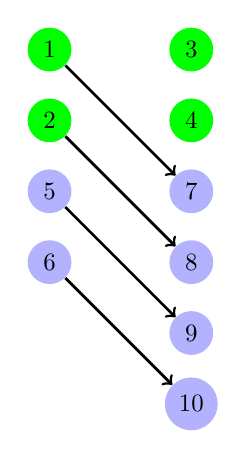
\begin{tikzpicture}[scale=.9, transform shape]
               \tikzstyle{every node} = [circle, fill=blue!30]
                                                              %        \node[fill=green] (10) at (2, 5) {$10$};
                              \node[fill=green] (1) at (0,4) {$1$}; \node[fill=green] (3) at (2,4) {$3$};
               \node[fill=green] (2) at (0,3) {$2$};  \node[fill=green] (4) at (2,3) {$4$};
                                                                      \node (9) at (2, 0) {$9$};
                                                                      \node (10) at (2, -1) {$10$};
               \node (6) at (0,1) {$6$}; \node (8) at (2,1) {$8$};
               \node (5) at (0,2) {$5$};  \node (7) at (2,2) {$7$};
              \foreach \from/\to in {1/7,2/8,5/9,6/10}
                   \draw [line width=1pt,->] (\from) -- (\to);             \end{tikzpicture}
  \caption*{Pooled\\asam=173}\label{matchings}
\endminipage\hfill
\minipage{0.32\textwidth}\centering
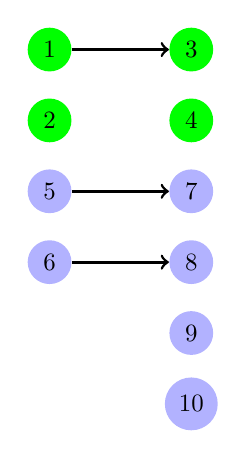
\begin{tikzpicture}[scale=.9, transform shape]
               \tikzstyle{every node} = [circle, fill=blue!30]
                                                              %        \node[fill=green] (10) at (2, 5) {$10$};
                              \node[fill=green] (1) at (0,4) {$1$}; \node[fill=green] (3) at (2,4) {$3$};
               \node[fill=green] (2) at (0,3) {$2$};  \node[fill=green] (4) at (2,3) {$4$};
                                                                      \node (9) at (2, 0) {$9$};
                                                                      \node (10) at (2, -1) {$10$};
               \node (6) at (0,1) {$6$}; \node (8) at (2,1) {$8$};
               \node (5) at (0,2) {$5$};  \node (7) at (2,2) {$7$};
              \foreach \from/\to in {1/3,5/7,6/8}
                   \draw [line width=1pt,->] (\from) -- (\to);             \end{tikzpicture}
  \caption*{Within\\ asam=115 }\label{matchings}
\endminipage\hfill
\minipage{0.32\textwidth}\centering
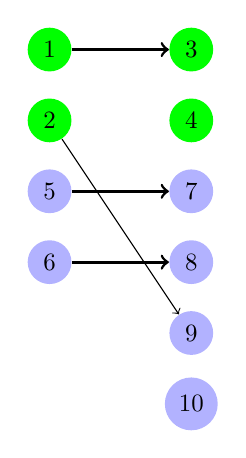
\begin{tikzpicture}[scale=.9, transform shape]
               \tikzstyle{every node} = [circle, fill=blue!30]
                                                              %        \node[fill=green] (10) at (2, 5) {$10$};
                              \node[fill=green] (1) at (0,4) {$1$}; \node[fill=green] (3) at (2,4) {$3$};
               \node[fill=green] (2) at (0,3) {$2$};  \node[fill=green] (4) at (2,3) {$4$};
                                                                      \node (9) at (2, 0) {$9$};
                                                                      \node (10) at (2, -1) {$10$};
               \node (6) at (0,1) {$6$}; \node (8) at (2,1) {$8$};
               \node (5) at (0,2) {$5$};  \node (7) at (2,2) {$7$};
              \foreach \from/\to in {1/3,5/7,6/8}
                   \draw [line width=1pt,->] (\from) -- (\to);
                                 \foreach \from/\to in {2/9}
                   \draw [black,->] (\from) -- (\to);
                          \end{tikzpicture}
\end{document}
